\section{Spread by RPKI class}\label{sec:prop}

We ask how much of the two-hour AS set of an origin change is visible at 30\,s.
We also ask how this share depends on the RPKI state of the new origin.
Measured from the first observation of the new origin, invalid origins show the largest share.
This difference is sensitive to where the onset falls, and catalogue selection also shapes it.

\begin{table}[t]
\small
\centering
\caption{Origin changes by year, catalogue population (2022: stratified sample only), ten collectors. First row: whole year, with the usable events of \Cref{tab:selection}. Other rows: test split. Upper rows: \floor $\Jac(\set{30s},\set{2h})$ with the onset at the first observation of the new origin. Middle rows: share of test events whose new origin was first observed at most 60\,s before the identifier, and the floor of these events. Lower rows: stratified sample and label-free invalid stratum. 2026 covers January to August.}
\label{tab:prop-summary}
\setlength{\tabcolsep}{3.2pt}
\begin{tabular}{lrrrrr}
\toprule
 & 2022 & 2023 & 2024 & 2025 & 2026 \\
\midrule
invalid share, year (\%) & 6.0 & 50.0 & 46.3 & 38.8 & 32.7 \\
\midrule
test events & 577 & 2,710 & 7,363 & 5,463 & 3,672 \\
\quad invalid & 31 & 1,419 & 3,725 & 2,290 & 1,455 \\
\quad unknown & 369 & 1,086 & 3,410 & 2,871 & 1,714 \\
\quad valid & 177 & 205 & 228 & 302 & 503 \\
$\Jac$, all events & 0.41 & 0.57 & 0.66 & 0.59 & 0.50 \\
\quad invalid & 0.47 & 0.66 & 0.74 & 0.71 & 0.61 \\
\quad unknown & 0.44 & 0.50 & 0.60 & 0.51 & 0.47 \\
\quad valid & 0.36 & 0.36 & 0.32 & 0.42 & 0.33 \\
\midrule
\multicolumn{6}{@{}l}{\emph{onset at most 60\,s before the identifier}} \\
share, invalid (\%) & 84 & 87 & 94 & 91 & 84 \\
\quad unknown (\%) & 47 & 57 & 71 & 62 & 59 \\
\quad valid (\%) & 33 & 36 & 41 & 46 & 28 \\
$\Jac$, invalid & 0.52 & 0.73 & 0.78 & 0.76 & 0.68 \\
\quad unknown & 0.70 & 0.75 & 0.80 & 0.69 & 0.73 \\
\quad valid & 0.74 & 0.64 & 0.54 & 0.69 & 0.63 \\
\midrule
stratified sample & 0.41 & 0.42 & 0.43 & 0.42 & 0.37 \\
label-free invalid & 0.51 & 0.50 & 0.55 & 0.49 & 0.58 \\
\quad onset near identifier & 0.61 & 0.62 & 0.67 & 0.64 & 0.68 \\
\bottomrule
\end{tabular}
\end{table}
% src: upper and lower rows: paper/generated/propagation-facts.json (scripts/paper_propagation_tables.py).
%   the annual "usable events" row (1,963 / 8,200 / 18,350 / 22,921 / 14,500) moved out: it repeats tab:selection (usable origin changes);
%   test events = propagation-facts.json years.Y.paper.test (= onset_sensitivity.json years.Y.all.pooled.test);
%   per-class test events (round 7, criterion M22(a); they replace the row "invalid share, test"): onset_sensitivity.json
%   years.Y.all.{invalid,unknown,valid}.test (31/369/177, 1,419/1,086/205, 3,725/3,410/228, 2,290/2,871/302, 1,455/1,714/503).
%   middle rows and "onset near identifier": paper/generated/onset_sensitivity.json and onset_sensitivity_ci.json
%   (scripts/paper_onset_sensitivity.py, scripts/paper_onset_sensitivity_ci.py; same inputs, hash-checked; test split).

\begin{figure*}[t]
\centering
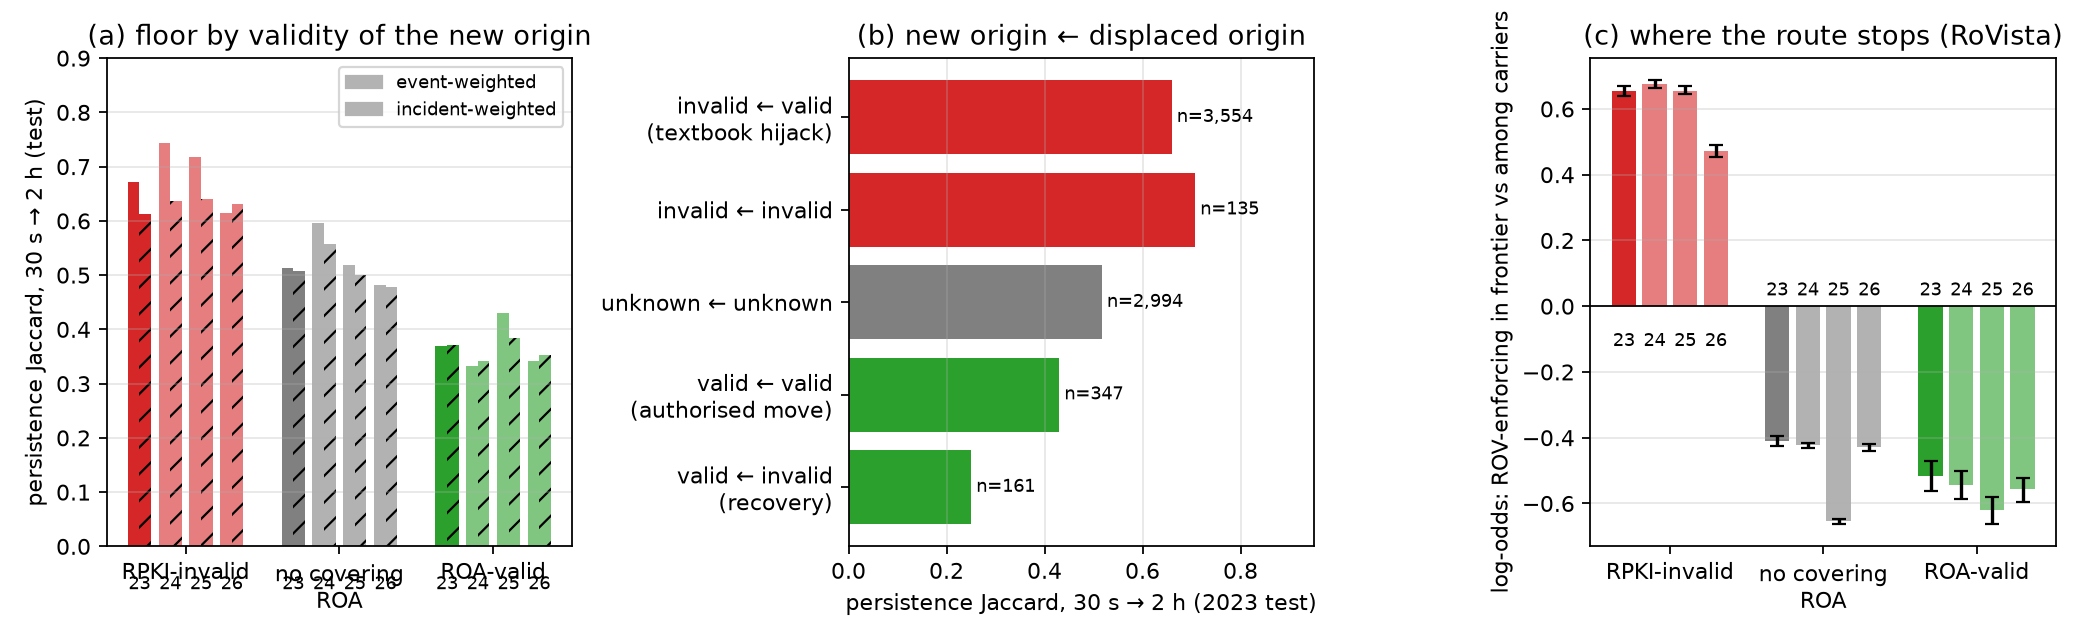
\includegraphics[width=\linewidth]{figures/rpki/rpki_headline}
\caption{Spread by RPKI class, catalogue population. (a, b) Test splits. (c) All usable events of each year. (a) \floor at 30\,s by validity of the new origin, with the onset at the first observation of the new origin (filled markers) and for events first observed at most 60\,s before the identifier (open markers). (b) Share of events whose new origin was observed more than 60\,s before the identifier. (c) Mean log-odds of the RoVista-protected share among non-carrying neighbours against carriers, by class and year, with 95\,\% event-bootstrap intervals that ignore clustering in days (hidden behind the marker where narrower); 2025 and 2026 use RoVista data up to May 2025.}
\Description{Three panels. With the onset at the first observation, invalid-origin events have the highest floor; for events first observed near the identifier, the differences between the classes in 2023--2026 are smaller, and this subset keeps far fewer valid than invalid events. Valid and unknown origins are often observed long before the identifier. Invalid-origin events have positive frontier log-odds, valid and unknown origins negative ones.}
% src: panel (c) population: paper/generated/frontier_facts.json uses all usable events of a year (2024 invalid 8,492, not the 3,725 test events; round-2 review, Figure 1 caption)
\label{fig:headline}
\end{figure*}

\paragraph{Floors from the first observation.}
With the onset at the first observation, the mean \floor of the catalogue population is 0.57 / 0.66 / 0.59 / 0.50 in 2023--2026 (\Cref{tab:prop-summary}).
Invalid-origin events have the highest floor in every year: 0.61--0.74 in 2023--2026, against 0.47--0.60 for unknown and 0.32--0.42 for valid origins (\Cref{fig:headline}a).
With UTC-day blocks, the differences invalid minus unknown and invalid minus valid have intervals above zero in 2023--2026.
The pooled floor follows the composition of the test split, whose invalid share falls from 52\,\% in 2023 to 40\,\% in 2026.
Year differences, above all against 2024, also compare two allowlist settings (\Cref{sec:data}).
The stratified sample, which depends less on the catalogue, has a floor of 0.41--0.43 in 2022--2025 and 0.37 in 2026.
% src: paper/generated/onset_sensitivity_ci.json years.*.all (day-block intervals, 2,000 repetitions); propagation-facts.json
% src (round 6, panel-r6 NEW-5, T5; DA #4): paper/generated/allowlist_by_year.json by_year.2024 {rule flat, thresholds_bins [50]},
%   by_year.{2022,2023,2025,2026} {rule per_week_scaled, thresholds_bins [200, 214, 221]} (sections/03-data.tex "Event identification"); the
%   within-year class orderings use one setting per year and are not affected.

\paragraph{Where the onset falls.}
The replay searches the new origin from one hour before the identifier (\Cref{sec:data}).
For invalid origins, the first observation is usually the identified change itself, with a median lag of 0\,s.
Valid and unknown origins often appear earlier, and valid origins have median lags of $-700$ to $-1{,}800$\,s over all events of a year.
We did not compute incident-weighted floors, because the event tables hold no incident identifier.
% src (round 8, criterion M11): data/corrected-release-20261016/eventset/<year>/events.parquet columns (no incident identifier).

In 2023--2026, the new origin was visible more than 60\,s before the identifier for 54--72\,\% of valid events.
The share is 29--43\,\% for unknown and 6--16\,\% for invalid events (\Cref{fig:headline}b).
Such an origin was already present at some collector peers, for example as a second origin of the prefix.
Its 30-s set can precede the identified change, which lowers the floor.
% src: paper/generated/propagation-facts.json years.*.paper.validity.*.observation_lag_s_p10_p50_p90; onset_sensitivity_ci.json share_near

\paragraph{Events with the onset near the change.}
We repeat the comparison for events first observed at most 60\,s before the identifier, the onset rule of the slow-regime forecasts (\Cref{sec:forecast-legacy}).
% round 6 (review-r6 W5 item 5, "the rule we also use for leaks"; panel-r5 NEW-13): only the slow regime applies this rule
%   (sections/08-forecast.tex "Task and candidates"; src/bgbench/baselines_eventset.py and curve_eventset.py filter observation_lag_s >= -60);
%   the R1/R2 manifests record observation_lag_s without a filter (src/bgbench/forecast_protocol.py), so R1 and R2 keep earlier events.
This rule keeps 84--94\,\% of invalid events but only 28--46\,\% of valid ones, so it selects differently by class.
In 2023--2026 it leaves \num{1228}--\num{3487} invalid, 621--\num{2410} unknown and 74--141 valid test events per year.
Our tables hold the sets only at fixed horizons, so we cannot move the other onsets.

For these events, invalid and unknown origins have floors of 0.68--0.78 and 0.69--0.80 in 2023--2026.
Invalid minus unknown is $-0.05$ to $+0.07$, and its day-block interval includes zero in 2023, 2024 and 2026, and is [$+0.01$, $+0.12$] in 2025.
Invalid minus valid is $+0.10$ [$+0.03$, $+0.17$] in 2023 and $+0.24$ [$+0.12$, $+0.35$] in 2024, against $+0.31$ and $+0.42$ from the first observation.
Its intervals include zero in 2025 and 2026, and in 2022 the ordering reverses, with invalid origins lowest (0.52, 26 test events).
Unknown minus valid is $+0.10$ to $+0.25$ in 2023, 2024 and 2026, with intervals above zero, and about zero in 2025.
The rule also changes which events each class keeps, so it does not isolate an effect of the onset.
% src (round 6, panel-r5 W8 / Q17, panel-r6 S17 "per-class n", "unknown-minus-valid near onset"): paper/generated/onset_sensitivity.json
%   years.{2023..2026}.near.{invalid,unknown,valid}.test: invalid 1,230 / 3,487 / 2,084 / 1,228, unknown 621 / 2,410 / 1,773 / 1,009, valid 74 / 93 / 138 / 141;
%   onset_sensitivity_ci.json years.*.near["unknown-valid"]: 2023 +0.1161 [0.0361, 0.1942], 2024 +0.2545 [0.1438, 0.3543], 2025 -0.0005
%   [-0.0788, 0.1085], 2026 +0.0952 [0.0244, 0.1688] (2022 -0.0342 [-0.1135, 0.05]). Per-class n rows are in tab:prop-summary (round 7). Not done: an
%   incident-weighted floor (the event tables hold no incident identifier).
% src: paper/generated/onset_sensitivity_ci.json years.*.near; onset_sensitivity.json (test n near: invalid 26 / 1,230 / 3,487 / 2,084 / 1,228; valid 59 / 74 / 93 / 138 / 141)
%   near invalid-unknown 2025: 0.0687 [0.0113, 0.1217]; near invalid-valid 2023: 0.0968 [0.027, 0.173], 2024: 0.2407 [0.1211, 0.3498],
%   2025: 0.0682 [-0.0218, 0.1795], 2026: 0.0421 [-0.0322, 0.1205]; all invalid-valid 2023: 0.3076, 2024: 0.4242 (years.*.all).

From the first observation, the ordering invalid $>$ unknown $>$ valid also holds at each collector in every year.
In 2024 it holds among /24 prefixes and in every bucket of origin customer cone and provider count.
These controls share the onset definition, so they do not remove its effect.

\paragraph{The catalogue shapes the invalid class.}
Radar labels 96--99\,\% of the invalid events of the catalogue population, but only 10--36\,\% of its valid events.
The label-free invalid stratum removes this selection.
Its floor is 0.49--0.58, and 0.61--0.68 for events with the onset near the identifier.
This is 0.11--0.12 below the catalogue invalid events with the same onset rule in 2023--2025, and equal in 2026.
The stratum comes from smaller origins, with a median customer cone of 2--3 ASes against 6--10 for labelled invalid events.
More of it is ROA-valid 7 or 30 days later, 25\,\% in 2023 rising to 36\,\% in 2026, against 7--11\,\% of the labelled invalid events.
% src: paper/generated/propagation-facts.json (labelled shares; stratum floors; cones; follow-up validity); onset_sensitivity.json (stratum_near; near invalid floors)

\paragraph{Catalogue tags.}
The RPKI tag of Radar agrees with our same-day validation on 93.0\,\% of \num{16739} matched events in 2024, and on 78.4\,\% of \num{21076} in 2025.
Without one mass event of AS53013 on 2025-05-28, it is 89.0\,\% in 2025.
Most disagreements are unknown in our data and invalid in Radar.
Anchor gaps cannot explain them in 2025, which has none, and in 2024 they cover five days and change one replayed event (\Cref{sec:data}).
% round 6 (panel-r6 NEW-6 / X2): "one replayed label" -> "one replayed event" (both neighbouring days agree; event 20240329T052152_154.203.175.0-24_138915
%   changes its new and its displaced origin); roa_anchor_check.json label_changes_by_group.2024 also holds one change under one repair only
%   (20240117T072525_102.129.203.0-24_395517, invalid -> invalid / valid).
% src (round 5, panel-r5 NEW-10 / domain B3; revision analysis): paper/generated/roa_anchor_check.json development.event_days_by_year:
%   2025 days_checked 365 (every calendar day), days_resolving_to_flagged_file 0; 2024 days_resolving_to_flagged_file 5 (all AFRINIC short,
%   tal_0.5_to_0.9_of_local_median: 2024-01-17, 01-25, 03-29, 04-26, 06-03), events_on_flagged_files 387 replayed events;
%   revalidation_on_flagged_files.assessment.by_group.2024 {"unknown->invalid": 1} (both repairs agree; event 20240329T052152_154.203.175.0-24_138915).
%   The file covers the replayed events, not the Radar-matched populations of radar_rpki_agreement (16,739 / 21,076), so for 2024 the anchor gaps
%   can explain at most the matched events of these five days; the 2025 statement holds for any population because no 2025 day file is flagged.
None of the \num{85639} Radar events carries a new-origin-valid tag, which fits its scoring design~\cite{li2026demystifying}.
% src: docs/paper/corrections-2026-10-16/ (radar_rpki_agreement); scripts/radar_rpki_agreement.py

\paragraph{The ROV frontier.}
RoVista~\cite{li2023rovista,rovista_data} measures with data-plane probes how often an AS cannot reach RPKI-invalid prefixes.
We call a measured AS \emph{RoVista-protected} when its latest ratio, dated at or before the event, is at least 0.5.
Protection can come from the AS itself or from an upstream~\cite{li2026rscope}.
In mid-2025, RoVista's median probes per AS and day fell from 10 in January to 5 in June and 1--2 from December.
% src (round 7, review-r6 W5 "dated, sourced probe counts"): docs/results/2026-09-15-extension-2022-2026.md "RoVista changed regime in
%   mid-2025" table (median `total` per AS-day: 2023-01 26, 2024-01 29, 2025-01 10, 2025-06 5, 2025-12 2, 2026-06 2, 2026-08 1; share >= 0.5
%   0.160 in 2025-01, 0.272 in 2025-06).
With this change, the protected share rose from 0.16 to 0.27 in one step.
We therefore keep each AS at its last ratio before 31 May 2025 for later events.

For each event, the carriers are the ASes on observed paths to the new origin within two hours.
The frontier holds their CAIDA one-hop neighbours that are not carriers.
Each event gets the log-odds of the protected share in its measured frontier relative to its measured carriers, adding one half to each cell.

In the catalogue population of 2023--2026, the mean is $+0.41$ to $+0.67$ for invalid origins and negative for valid and unknown origins (\Cref{fig:headline}c).
Invalid minus valid is $+1.10$ to $+1.30$, and invalid minus unknown $+1.00$ to $+1.34$.
In 2022, whose invalid events come mostly from the label-free stratum, these values are $+0.31$, $+0.96$ and $+1.01$.
The label-free stratum has smaller means, $+0.12$ to $+0.19$.
Its log-odds is negative if we pool its AS--event observations and do not average per event, so its sign depends on the aggregation.

RoVista measures 38--51\,\% of frontier ASes and 57--72\,\% of carriers.
The event-bootstrap intervals in \Cref{fig:headline}c ignore that events cluster in incidents and days, so we use the frontier only descriptively.
Carriage of an invalid route and a RoVista probe both depend on whether an AS reaches invalid prefixes.
The frontier is a consistency check between passive and active data, not independent evidence of ROV.
% src: paper/generated/frontier_facts.json; generated/frontier.tex; generated/frontier_diff.tex
%   (round-3 reviews: panel M7, second reviewer W3: frontier kept descriptive; the "intervals above zero" wording was removed, every value is unchanged).

\paragraph{Route leaks.}
Leaks keep a high floor of 0.69 / 0.71 / 0.69 over all usable leaks of 2024 / 2025 / 2026.
The floor is 0.77 in 2024 and 0.74 in 2025 for leaks whose observed onset is at most 60\,s before the identifier.
The 396 leaks per year of 2022 and 2023 are large by construction and volume-selected only (\Cref{tab:leak-audit}), with floors of 0.42 and 0.44.
Leaks that reach 200 or more ASes are the open problem, where \Cref{sec:forecast} starts.
% src: paper/generated/propagation-facts.json years.*.leak
